\documentclass[a4paper, notitlepage, 12pt]{scrartcl}
\author{Lukas Rost \\ \small{Teilnahme-ID: 48125}}
\title{Aufgabe 1 \\ \glqq Lisa rennt\grqq  - Dokumentation}
\subtitle{37. Bundeswettbewerb Informatik 2018/19 - 2. Runde \\~\\}
\date{29. April 2019}
\usepackage[ngerman]{babel}
%\usepackage[utf8]{inputenc}
\usepackage{graphicx}
\usepackage{wrapfig}
\usepackage{color}
\usepackage[dvipsnames]{xcolor}
\usepackage{hyperref}
\usepackage[top=2.5cm, bottom=1.5cm, left=2.5cm, right=2.5cm]{geometry}
\usepackage{fancyvrb}
\usepackage{caption}
\usepackage{mathtools}
\usepackage{amssymb}
\usepackage{fancyhdr}
\usepackage{lastpage}
\usepackage{algorithm}
\usepackage{algpseudocode}

\usepackage{minted}
\fvset{breaklines=true}

\pagestyle{fancy}
\lhead{Lukas Rost, Teilnahme-ID: 48125}
\rhead{Aufgabe 1, Seite \thepage ~von \pageref{LastPage}}
\cfoot{ }

\newenvironment{longlisting}{\captionsetup{type=listing}}{}

\newmintedfile{python}{frame=single,linenos,samepage=false,firstnumber=1,rulecolor=\color{Gray},autogobble,breakafter=.,fontsize=\small}

\floatname{algorithm}{Algorithmus}

\newcount\colveccount
\newcommand*\colvec[1]{
	\global\colveccount#1
	\begin{pmatrix}
		\colvecnext
	}
	\def\colvecnext#1{
		#1
		\global\advance\colveccount-1
		\ifnum\colveccount>0
		\\
		\expandafter\colvecnext
		\else
	\end{pmatrix}
	\fi
}


\begin{document}
\renewcommand{\contentsname}{\centerline{Inhaltsverzeichnis}}
 \maketitle
 \tableofcontents
 \thispagestyle{empty}
 \newpage
 \setcounter{page}{1}
 
 \section{Lösungsidee}
 \subsection{Das Geometric-Shortest-Path-Problem}
 Das der Aufgabe zugrundeliegende Problem nennt sich \textit{Geometric Shortest Path} (GSP), auf Deutsch auch bekannt als Problem des geometrischen kürzesten Weges. Bei diesem Problem ist ein punktförmiger Roboter (oder auch eine Schülerin namens Lisa) gegeben, der/die sich an einer Startposition $p_{start}$ in einem kartesischen Koordinatensystem befindet. In diesem Koordinatensystem befinden sich mehrere als Polygone modellierte Hindernisse, wobei jedes einzelne Polygon durch seine Eckpunkte gegeben ist.\footnote{In dieser Dokumentation wird angenommen, dass die Punkte entgegen dem Uhrzeigersinn sortiert sind, sonst muss dies vorher geschehen.} Weiterhin ist eine Position $p_{ziel}$ gegeben. Nun soll ein möglichst kurzer Weg von $p_{start}$ zu $p_{ziel}$ gefunden werden, wobei dieser nicht durch Hindernisse führen soll.\footnote{Zumindest nicht, wenn Lisa als Zielposition nicht das Krankenhaus erreichen will.}\cite{Src:noem} \\ \\
 Das hier gegebene Problem unterscheidet sich von GSP dadurch, dass keine Position $p_{ziel}$, sondern ein Strahl $s_{ziel}$ (in Form eines beliebigen Punktes auf dem Strahl) erreicht werden soll. In diesem Fall handelt es sich dabei um die y-Achse ($x=0$ mit $y \geq 0$). Zusätzlich soll nicht unbedingt der Weg optimiert werden, sondern die Startzeit, die abhängig von der Länge des Weges und der für jeden Punkt des Strahls unterschiedlichen Zielzeit ist. Diese Zielzeit kann mithilfe des Abstands des Punktes vom Ursprung berechnet werden. \\ \\
 Das Geometric-Shortest-Path-Problem wird im Allgemeinen in zwei Schritten gelöst: Zunächst wird ein Sichtbarkeitsgraph erstellt, auf welchem dann Dijkstras Algorithmus ausgeführt wird. Zur Lösung des hier gegebenen Problems wird jedoch ein zusätzlicher Schritt benötigt, der auf der Lösung des Problems ohne Hindernisse basiert. Diese drei Algorithmen sollen in den folgenden Abschnitten vorgestellt und näher erläutert werden.
 \begin{figure}[H]
 	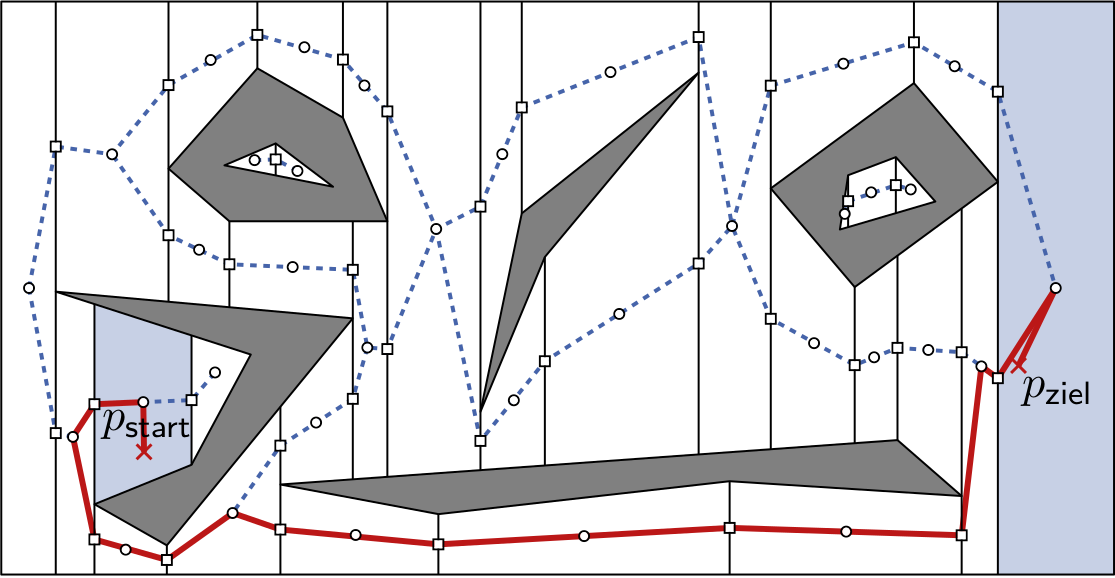
\includegraphics[scale=0.41]{pics/gsp}
 	\caption{Illustration des GSP-Problems (aus \cite{Src:noem})}
 \end{figure}
 \subsection{Erzeugung eines Sichtbarkeitsgraphen}
 Es lässt sich beobachten, dass der kürzeste $s$-$t$-Weg (dabei sei $s$ die Startposition und $t$ die Zielposition) in einem solchen Koordinatensystem ein Polygonzug sein muss, dessen innere Knoten Knoten (bzw. Ecken) der Hindernisse sind. Andernfalls wäre es immer möglich, einen kürzeren Weg zu konstruieren, der über einen Hindernisknoten führt.\cite{Src:noem} Ausgehend davon lässt sich ein sogenannter Sichtbarkeitsgraph erzeugen, bei dem es sich um einen gewichteten, ungerichteten Graphen handelt. \\ \\
 Für eine Polygonmenge $S$ mit Knotenmenge $V(S)$ sei dieser definiert als $G_{vis}(S) = (V(S),E_{vis}(S))$. Dabei ist $E_{vis}(S)$ die Menge der Knotenpaare von $S$, sodass die dazwischenliegende Strecke kein Polygon (bzw. das Innere eines Polygons) schneidet. Mathematisch ausgedrückt bedeutet das $E_{vis}(S) = \{ uv | u,v \in V(S)$ und $\overline{uv} \subset C_{free} = \mathbb{R}^{2} \setminus \bigcup S \}$. Das Gewicht einer Kante sei dabei als euklidischer Abstand der beiden Endpunkte definiert. \\ \\
 Wenn man $S^{*}$ als $S \cup \{s\}$ definiert (bei normalen Sichtbarkeitsgraphen wird auch $t$ hinzugefügt) und den Sichtbarkeitsgraphen dafür analog, kann man damit das GSP-Problem lösen. Nun entspricht der kürzeste $s$-$t$-Weg, der Hindernisse vermeidet, einem kürzesten Weg in $G_{vis}(S^{*})$.
 \subsubsection{Naiver Ansatz}
 $G_{vis}(S^{*})$ lässt sich nun naiv in $\mathcal{O}(n^3)$ berechnen, wobei $n = |V(S^*)|$. Dazu bestimmt man für jeden Knoten $u \in V(S*)$ die von ihm sichtbaren Knoten $v$. Dabei muss man für jede Strecke $\overline{uv}$ prüfen, ob sie eine der $|E_{vis}(S^*)| = \mathcal{O}(n)$ in Frage kommenden Hinderniskanten schneidet. Die Bestimmung der von $u$ sichtbaren Knoten ist somit in $\mathcal{O}(n^2)$ durchführbar und insgesamt ergibt sich eine Laufzeit von $O(n^3)$. \\ \\
 Die Funktionsweise des naiven Algorithmus wird auch in folgendem Pseudocode deutlich: 
 \begin{algorithm}[H]
 \begin{algorithmic}
 	\Function{visibilityGraph}{$S$}
 	\State $G = (V(S),E) \gets$ leerer Sichtbarkeitsgraph
 	\ForAll{Knoten $v \in V(S)$}
 	\Comment{\small{$\mathcal{O}(n)$}}
 	\ForAll{Knoten $w \in V(S) \setminus \{ v \}$}
 	\Comment{\small{$\mathcal{O}(n)$}}
 	\ForAll{Kante $e \in E_{vis}(S)$}
 	\Comment{\small{$\mathcal{O}(n)$}}
 	\If{$\overline{vw}$ schneidet keine der Kanten $e$}
 	\State $E \gets E \cup \{vw\}$
 	\EndIf
 	\EndFor
 	\EndFor
 	\EndFor
 	\State \Return $G$
 	\EndFunction
 \end{algorithmic}
\caption{Naiver Algorithmus}
\end{algorithm} ~\\
 \subsubsection{Der Lee-Algorithmus}
 Es ist jedoch auch möglich, die Bestimmung der von $u$ sichtbaren Knoten in $\mathcal{O}(n \cdot \log n)$ durchzuführen, wodurch sich insgesamt eine Laufzeit von $\mathcal{O}(n^2 \cdot \log n)$ ergibt. Der dazu notwendige Algorithmus ist der Algorithmus von D. T. Lee. Durch dessen geringere Laufzeit lässt sich insbesondere bei großen Eingaben eine deutliche Verbesserung erreichen. \\ \\
 Es existieren zwar noch schnellere Algorithmen wie der nach Overmars und Welzl in $\mathcal{O}(n^2)$ oder der nach Ghosh und Mount in $\mathcal{O}(n \cdot \log n + E)$\cite{Src:kitz}. Doch die damit erreichten Verbesserungen sind nur in speziellen Fällen wirklich bemerkbar, während die Implementierung deutlich schwieriger ist. \\ \\
 Lees Algorithmus ist grundlegend ähnlich aufgebaut, muss jedoch für jede Strecke $\overline{uv}$ nur noch eine Hinderniskante prüfen, welche in $\mathcal{O}(\log n)$ bestimmt werden kann. Dies wird auch in folgendem Pseudocode deutlich:
 \begin{algorithm}[H]
 \begin{algorithmic}
 	\Function{visibilityGraph}{$S$}
 	\State $G = (V(S),E) \gets$ leerer Sichtbarkeitsgraph
 	\ForAll{Knoten $v \in V(S)$}
 	\Comment{\small{$\mathcal{O}(n)$}}
 	\State $W \gets$ \Call{visible\_vertices}{v,S}
 	\Comment{\small{$\mathcal{O}(n \cdot log~n)$}}
 	\State $E \gets E~ \cup \{vw~|~w \in W \}$
 	\EndFor
 	\EndFunction
 \end{algorithmic}
 \caption{Der Algorithmus von Lee}
 \end{algorithm}
 Der Algorithmus in der Methode \texttt{visible\_vertices} benutzt dabei eine sogenannte rotierende \emph{Sweep line} beziehungsweise \emph{Scan line}. Diese Sweep line fegt (\glqq sweept\grqq) den zweidimensionalen Raum aus, wobei sie durch den gesamten Raum bewegt wird, bis alle Objekte (in diesem Fall die Knoten) besucht und verarbeitet wurden. Im Falle von Lees Algorithmus rotiert die Sweep line (mathematisch gesehen ein Strahl) um dem Startpunkt $v$ gegen den Uhrzeigersinn. \\ \\
 Am Anfang zeigt die Sweep line nach rechts (parallel zur x-Achse) und rotiert so lange gegen den Uhrzeigersinn, bis sie einen Punkt trifft, der auf Sichtbarkeit überprüft werden muss. Dazu wird eine Liste der offenen Kanten geführt, mit denen sich die Sweep line aktuell überhaupt schneiden kann und die damit relevant sind.\cite{Src:pyvistwo} Anfangs werden dabei einmal alle Kanten daraufhin überprüft, ob sie sich mit der Sweep line (in der Anfangsstellung) schneiden. Entsprechend wird dann diese Liste initialisiert. \\ \\
 Trifft die Sweep line auf einen Punkt $a$, werden deshalb alle Kanten überprüft, deren Endpunkt $a$ ist. Liegt eine Kante bezüglich der Sweep line im Uhrzeigersinn (\emph{clockwise side}), kann sie, sofern sie enthalten ist, aus der Liste der offenen Kanten entfernt werden, da die Sweep line bei Bewegung gegen den Uhrzeigersinn nie wieder mit ihr in Berührung kommt. Liegt die Kante dagegen entgegen des Uhrzeigersinns (\emph{counter-clockwise side}), so muss sie zu den offenen Kanten hinzugefügt werden, da sich die Sweep line im Folgenden mit ihr schneiden kann. \\ \\
 So werden in diesem Beispiel (siehe nächste Seite) am Punkt $a$ die Kanten $\overline{ab}$ und $\overline{ac}$ hinzugefügt, da sie bezüglich der Sweep line gegen den Uhrzeigersinn (auf ihrer linken Seite) liegen. In Punkt $b$ kann $\overline{ab}$ dagegen wieder entfernt werden, da sie rechts der Sweep line liegt. Hier wird dann jedoch $\overline{bc}$ hinzugefügt.
  \begin{figure}[H]
 	\centering 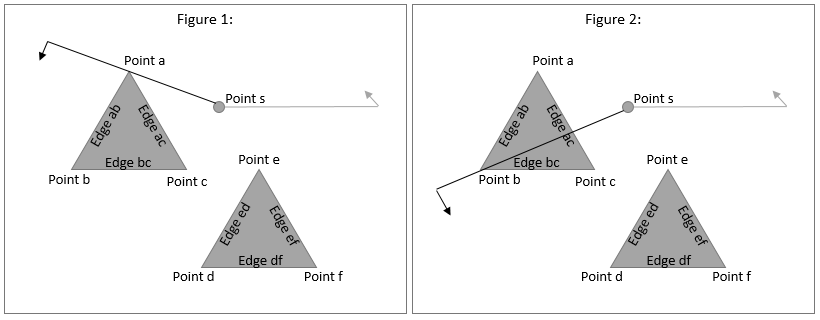
\includegraphics[scale=0.6]{pics/lee_figure1}
 	\caption{Illustration des Konzepts der \emph{Sweep line} (aus \cite{Src:pyvistwo})}
 \end{figure}
Es lässt sich zeigen, dass sogar nur diejenige offene Kante geprüft werden muss, welche am nächsten an $v$ liegt, d.h. diejenige, für die der Schnittpunkt mit der Sweep line am nächsten an $v$ liegt. Um diese Kante schnell zu bestimmen, muss man die Kanten nach der Distanz zum Schnittpunkt ordnen. Dies lässt sich zum Beispiel mit einem balancierten binären Suchbaum wie einem \emph{AVL-Baum} erreichen.\cite{Src:pyvistwo} \\ \\
Die \texttt{visible\_vertices}-Funktion sieht nun also bei einer Formulierung als Pseudocode ungefähr so aus:
\begin{algorithm}[H]
\begin{algorithmic}
	\Function{visible\_vertices}{$v,S$}
	\State $w \gets sort(V(S) \setminus \{v\} )$
	\Comment{Sortieren der Knoten (siehe unten)}
	\State $s \gets v + \lambda \cdot \colvec{2}{1}{0}$ mit $\lambda \in \mathbb{R}^+$
	\Comment{Sweep line initialisieren}
	\State{$T \gets binarySearchTree()$}
	\State{$W \gets \emptyset$}
	\ForAll{Kante $e \in E(S)$}
	\If{$e \cap s \neq \emptyset$}
	\Comment{alle Kanten, die die Sweep line schneiden}
	\State{$T \gets T \cup e$}
	\EndIf
	\EndFor
	\ForAll{Knoten $w_i \in w$}
	\Comment{in sortierter Reihenfolge}
	\State{Rotiere $s$ so, dass er $w_i$ schneidet}
	\If{\Call{visible}{$w_i$}}
	\Comment{ist sichtbar}
	\State{$W \gets W \cup w_i$}
	\EndIf
	\ForAll{Kante $e$ mit Endpunkt $w_i$}
	\If{$e$ links von $s$}
	\State{$T \gets T \cup \{e\}$}
	\Comment{Kante hinzufügen}
	\EndIf
	\If{$e$ rechts von $s$}
	\State{$T \gets T \setminus \{e\}$}
	\Comment{Kante entfernen}
	\EndIf
	\EndFor
	\EndFor
	\State{\Return $W$}
	\EndFunction
\end{algorithmic}
\caption{Bestimmung der sichtbaren Knoten bzw. Punkte im Lee-Algorithmus}
\end{algorithm}
Das Sortieren der Knoten erfolgt dabei anhand ihrer Polarkoordinaten relativ zu $v$. Dabei wird zuerst nach kleinerem Winkel zu $s$ und dann, falls dieser gleich sein sollte nach kleinerem Abstand zu $v$ sortiert. Die Formulierung \emph{links} im Pseudocode bedeutet entgegengesetzt dem Uhrzeigersinn und \emph{rechts} bedeutet im Uhrzeigersinn. \\
\begin{algorithm}[H]
\begin{algorithmic}
	\Function{visible}{$w_i$}
	\If{$ T = \emptyset$}
	\State \Return true
	\EndIf
	\If{$\overline{vw_i} \cap smallest(T) = \emptyset$}
	\State \Return true
	\Else
	\State \Return false
	\EndIf
	\EndFunction
\end{algorithmic}
\caption{Sichtbarkeitsprüfung im Lee-Algorithmus}
\end{algorithm}
Diese Funktion \texttt{visible} prüft dabei ganz einfach die Sichtbarkeit eines Knotens. $smallest(T)$ gibt die kleinste Kante im Suchbaum an.
 \subsection{Der Dijkstra-Algorithmus}
 Um nun im Sichtbarkeitsgraphen einen kürzesten Pfad vom Startknoten $s$ zu allen anderen Knoten zu bestimmen, was für die Lösung des Problems notwendig ist, kann man Dijkstras Algorithmus verwenden. Dieser arbeitet nach dem Greedy-Prinzip, bei dem in jedem Schritt ein optimaler Folgezustand gewählt wird, der das aktuell beste Ergebnis verspricht. Er arbeitet grundlegend wie folgt:
 \begin{enumerate}
 	\item Weise allen Knoten die beiden Eigenschaften „Distanz“ und „Vorgänger“ zu. Initialisiere die Distanz im Startknoten $s$ mit 0 und in allen anderen Knoten mit $\infty$.
 	\item Solange es noch unbesuchte Knoten gibt, wähle darunter denjenigen mit minimaler Distanz aus und
 	\begin{enumerate}
 		\item speichere, dass dieser Knoten schon besucht wurde.
 		\item Berechne für alle noch unbesuchten Nachbarknoten die Summe des jeweiligen Kantengewichtes und der Distanz im aktuellen Knoten.
 		\item Ist dieser Wert für einen Knoten kleiner als die dort gespeicherte Distanz, aktualisiere sie und setze den aktuellen Knoten als Vorgänger.
 	\end{enumerate}
 \end{enumerate}
Der Dijkstra-Algorithmus hat eine Laufzeit von $\mathcal{O}((|V|+|E|) \cdot \log |V|)$ (bei Implementierung mit einer Vorrangwarteschlange). Da der Algorithmus den entsprechenden Weg durch das Setzen eines Vorgängers ebenfalls bestimmt, kann auch dieser selbst ausgegeben werden.
 \subsection{Lösung des Problems ohne Hindernisse}
 \subsection{Kombination der Ansätze}
 \subsection{Laufzeitbetrachtung}
 %TODO ausführlich
 \subsection{Erweiterungen}
 \subsubsection{Anpassbare Geschwindigkeiten}
 Es ist relativ einfach möglich, die Geschwindigkeiten, mit denen sich Lisa und der Bus bewegen, zu verändern. Dazu muss einfach in allen Gleichungen, die aus Weg und Geschwindigkeit die benötigte Zeit berechnen, die Geschwindigkeit entsprechend gewählt werden. Da bei der \emph{Lösung des Problems ohne Hindernisse} bereits die Geschwindigkeiten als Parameter verwendet wurden, ist dies auch dort ohne Probleme möglich. \\ \\
 Diese Erweiterung läuft in $\mathcal{O}(1)$ und wurde \textbf{implementiert} (siehe Umsetzung).
 \subsubsection{Andere Zielgeraden}
 Auch die Gerade bzw. der Strahl, auf der bzw. dem der Bus fährt, kann geändert werden. Dazu muss einfach das Koordinatensystem so transformiert werden, dass die Gerade im ursprünglichen Koordinatensystem der y-Achse im transformierten Koordinatensystem entspricht. Dies kann durch Drehungen und Parallelverschiebungen geschehen. \\ \\
 %TODO wie und algorithmus
 Die Erweiterung läuft pro Punkt in konstanter Laufzeit, also insgesamt in $\mathcal{O}(n)$. Diese Erweiterung wurde \textbf{implementiert}.
 %ggf. https://en.wikipedia.org/wiki/Translation_of_axes und https://en.wikipedia.org/wiki/Rotation_of_axes
  \subsubsection{Polygonale Lisa}
 Nun modellieren wir Lisa nicht mehr als Punkt, sondern als Polygon. Wieso? Möglicherweise handelt es sich bei einem der Hindernispolygone um das örtliche Fastfoodrestaurant und Lisa besucht dieses sehr oft, sodass sie extrem zugenommen hat. \\ \\
 Möglicherweise ist der Grund aber auch unspektakulärer. Eventuell ist Lisa gerade 18 geworden und möchte nun mit ihrem Auto zur Bushaltestelle fahren, auch wenn man über die ökologische Sinnhaftigkeit dieses Vorhabens streiten kann.\footnote{Hier Fridays-for-Future-Demonstration einfügen.} \\ \\
 Dies lässt sich mathematisch beschreiben, indem man für jedes Hindernispolygon dessen Minkowski-Summe mit dem Lisa-Polygon berechnet und auf den so entstandenen Polygonen den ursprünglichen Algorithmus ausführt. Die Minkowski-Summe ist dabei für zwei Teilmengen $A$ und $B$ (in diesem Fall Polygone) eines Vektorraums (des $\mathbb{R}^{2}$) definiert als:
 \begin{equation}
 A + B := \{a+b\,|\,a \in A, b \in B\}
 \end{equation}
 Sie ist also die Menge aller Elemente, die Summen von je einem Element aus $A$ und einem aus $B$ sind.\cite{Src:minkowski} Dies entspricht im Prinzip dem Entlangfahren des Lisa-Polygons am Rand des Hindernispolygons. Dabei wird das Hindernis so verbreitert, dass Lisa nun wieder als punktförmig angenommen und der ursprüngliche Algorithmus ausgeführt werden kann. \\ \\
 Seien nun das Hindernispolygon $P = (v_1,...,v_n)$ und das Lisa-Polygon $L = (w_1,...,w_m)$ mit $v_i$ und $w_i$ als Eckpunkten, wobei $v_1$ und $w_1$ die Punkte mit der minimalen y-Koordinate sind. Für diese zwei konvexen Polygone (im weiteren werden für diese Erweiterung nur solche betrachtet) im $\mathbb{R}^{2}$ kann die Minkowski-Summe wie folgt berechnet werden:
 \begin{algorithm}[H]
\begin{algorithmic}
	\Function{minkowskiSum}{$P$,$L$}
	\State $i \gets 1$; $j \gets 1$
	\State $v_{n+1} = v_1$; $w_{m+1} = w_1$
	\State $S = \emptyset$ \Comment{leeres Polygon}
	\Repeat
	\State $S = S \cup \{v_i + w_j\}$
	\If{\Call{winkel}{$v_i,v_{i+1}$} $<$ \Call{winkel}{$w_j,w_{j+1}$}}
	\State $i \gets i + 1$
	\EndIf
	\If{\Call{winkel}{$v_i,v_{i+1}$} $>$ \Call{winkel}{$w_j,w_{j+1}$}}
	\State $j \gets j + 1$
	\EndIf
	\If{\Call{winkel}{$v_i,v_{i+1}$} $=$ \Call{winkel}{$w_j,w_{j+1}$}}
	\State $i \gets i + 1$; $j \gets j + 1$
	\EndIf
	\Until{$i = n + 1$ and $j = m + 1$}
	\EndFunction
\end{algorithmic}
\caption{Bestimmung der Minkowski-Summe}
\end{algorithm}
\hspace*{-1em}Dieser Algorithmus läuft offensichtlich in $\mathcal{O}(n + m)$, denn $i$ wird höchstens $n$ Mal inkrementiert und $j$ $m$ Mal. Da er $n_{Polygon}$ Mal\footnote{Anzahl der Polygone} ausgeführt wird, erhält man $\mathcal{O}(n_{Polygon} \cdot (n + m)) = \mathcal{O}(n_{Orig} + n_{Polygon} \cdot m)$, wobei $n_{Orig}$ das ursprüngliche $n$ als Anzahl aller Eckpunkte aller Polygone ist. Diese Erweiterung wurde \textbf{implementiert}.
 \subsubsection{Nicht-polygonale Hindernisse}
 Es wäre auch möglich, die Art der Hindernisse auf Flächen, die keine Polygone sind, zu erweitern. Dies könnten beispielsweise Ovale oder Kreise sein. Eine Möglichkeit, den Sichtbarkeitsgraph darauf zu erweitern, ist in \cite{Src:arcvis} beschrieben. Dabei muss man anstelle des klassischen Sichtbarkeitsgraphen einen Tangenten-Sichtbarkeitsgraphen verwenden. Da dies jedoch relativ kompliziert ist, wird an dieser Stelle nicht genauer darauf eingegangen. \\ \\
 Diese Erweiterung wurde \textbf{nicht implementiert}.
 \subsubsection{Das Problem im $\mathbb{R}^{3}$}
 Nehmen wir nun an, dass Lisa fliegen kann. Wie sie diese Fähigkeit erlangt hat, ist unwichtig. Möglicherweise ist sie mit Quax aus der letztjährigen 3. Aufgabe der 2. Runde befreundet und kann seinen Quadrocopter benutzen. Außerdem nehmen wir an, dass der Bus unendlich hoch ist. Inwiefern das sinnvoll ist, soll hier ebenfalls nicht betrachtet werden. \\ \\
 Dazu kann man das Koordinatensystem von einem $\mathbb{R}^{2}$ auf einen $\mathbb{R}^{3}$ erweitern, sodass ein dreidimensionales Koordinatensystem entsteht. In diesem sind die Hindernisse dann Körper und die Zielgerade eine Zielebene, genauer die $yz$-Ebene. Ein Ansatz dazu ist in \cite{Src:3dvis} beschrieben. \\ \\
 Ein solcher Sichtbarkeitsgraph ist dann jedoch ein Hypergraph, bei dem jede Kante 3 Knoten verbindet. Aus diesem Grund wurde die Erweiterung \textbf{nicht implementiert}. 
\begin{thebibliography}{xx}
\bibitem[1] {Src:bit} Bittel, O. (HTWG Konstanz): Autonome Roboter - Wegekartenverfahren, SS 2016 (Präsentation), \url{http://www-home.htwg-konstanz.de/~bittel/msi_robo/Vorlesung/06_Planung_Wegekarten.pdf}
\bibitem[2] {Src:noem} Nöllenburg, Martin (KIT): Vorlesung Algorithmische Geometrie - Sichtbarkeitsgraphen, 2011 (Präsentation), \url{https://i11www.iti.kit.edu/_media/teaching/sommer2011/compgeom/algogeom-ss11-vl14-printer.pdf}
\bibitem[3]{Src:pyvis} Reksten-Monsen, Christian: Distance Tables Part 1 - Defining the Problem, \url{https://taipanrex.github.io/2016/09/17/Distance-Tables-Part-1-Defining-the-Problem.html}
\bibitem[4]{Src:pyvistwo} Reksten-Monsen, Christian: Distance Tables Part 2 - Lee's Visibility Graph Algorithm, \url{https://taipanrex.github.io/2016/10/19/Distance-Tables-Part-2-Lees-Visibility-Graph-Algorithm.html}
\bibitem[5]{Src:kitz} Kitzinger, John (University of New Mexico): The Visibility Graph Among Polygonal Obstacles: A Comparison of Algorithms, 2003, \url{https://www.cs.unm.edu/~moore/tr/03-05/Kitzingerthesis.pdf}
\bibitem[6]{Src:3dvis} Bygi, Mojtaba Nouri; Ghodsi, Mohammad (Sharif University of Technology): 3D Visibility Graph, \url{https://pdfs.semanticscholar.org/aba1/5853197c24ed6f164e4fb5e2f134462c7ebf.pdf}
\bibitem[7]{Src:LeeLee} Coleman, Dave (University of Colorado): Lee's Visibility Graph Algorithm - Implementation and Analysis, 2012, \url{https://github.com/davetcoleman/visibility_graph/blob/master/Visibility_Graph_Algorithm.pdf}
\bibitem[8]{Src:arcvis} Hutchinson, Joan P. (Macalester College): Arc- and circle-visibility graphs, \url{https://pdfs.semanticscholar.org/d257/d8f5ea2f9bb32c555b4d5723fdcf1e97dc4f.pdf}
\bibitem[9]{Src:minkowski} Skript der Uni Freiburg zur Minkowski-Summe, \url{http://algo.informatik.uni-freiburg.de/bibliothek/books/ad-buch/k7/slides/08.pdf}
\end{thebibliography}

\section{Umsetzung}
\subsection{Allgemeine Hinweise zur Benutzung}
\subsection{Struktur des Programms}
\subsection{Implementierung der wichtigsten Algorithmen}

\section{Beispiele}
\subsection{Beispiel 1}
\subsection{Beispiel 2}
\subsection{Beispiel 3}
\subsection{Beispiel 4}
\subsection{Beispiel 5}
\subsection{Eigene Beispiele}
\subsection{Beispiele für die Erweiterungen}

 \section{Quellcode}
 \renewcommand{\listingscaption}{Quellcode}
 
 \end{document}